\documentclass[11pt]{beamer}
\usetheme{Antibes}
\usepackage[utf8]{inputenc}
\usepackage[german]{babel}
\usepackage[T1]{fontenc}
\usepackage{amsmath}
\usepackage{amsfonts}
\usepackage{amssymb}
\usepackage{graphicx}
\usepackage{float}
\author{Gruppe C14 \\ Julián Häck, Martin Koytek, Lars Wenning, Erik Zimmermann}
\title{Bestimmen der Schallgeschwindigkeit über das Vermessen einer stehenden Welle}

\begin{document}

\section{Versuchsbeschreibung}
\begin{frame}
\begin{itemize}
\item $v_{Schall} = \lambda\cdot f$
\item messen des Schalldrucks um charakteristische Punkte der stehenden Welle aufzuzeichnen
\item Lineare Regression durchführen
\item $v_{Schall}$ aus Steigung der Linearen Regression bestimmen
\end{itemize}
\end{frame}

\section{Aufbau und Durchführung}
\begin{frame}{Aufbau}
\begin{figure}[H]
\centering
\includegraphics[scale=0.08]{Bilder/Druckknoten-Messung3.jpg}
\caption{Versuchsaufbau für die Bestimmung der Schallgeschwindigkeit über die Vermessung einer stehenden Welle}
\end{figure}
\end{frame}

\begin{frame}{Durchführung}
\begin{figure}[H]
\centering
\includegraphics[scale=0.25]{Bilder/baeuche.png}
\caption{Amplitude des Schalldrucks aufgetragen gegen eingeführte Länge des Richtmikrofons, $l = (0.025 + n\cdot 0.005) - 0.425$ in m}
\end{figure}
\end{frame}

\section{Auswertung}
\begin{frame}{Rohdaten}
\begin{table}[H]
\begin{tabular}{c|c|c}
Position Bauch N & Messpunkt n & Länge [m] \\ 
\hline 
1.5 & 1 & 0.395 \\ 
2.5 & 15 & 0.325 \\ 
3.5 & 30 & 0.25 \\ 
4.5 & 45 & 0.175 \\ 
\end{tabular}
\caption{Druckbäuche für $f = 2400\,$Hz, mit $\sigma_l = 0.0028\,$m}
\end{table}
\end{frame}

\begin{frame}{Transformation der Rohdaten}
\begin{figure}[H]
\centering
\includegraphics[scale=0.25]{Bilder/linreg_stehende_welle.eps}
\caption{Lineare Regression der 4 oben genannten Peaks, die Steigung beträgt $\frac{\lambda}{2}$, $\frac{\chi^2}{f} = 0.47$}
\end{figure}
\end{frame}

\begin{frame}{Auswertung der Anpassung}
\begin{figure}[H]
\centering
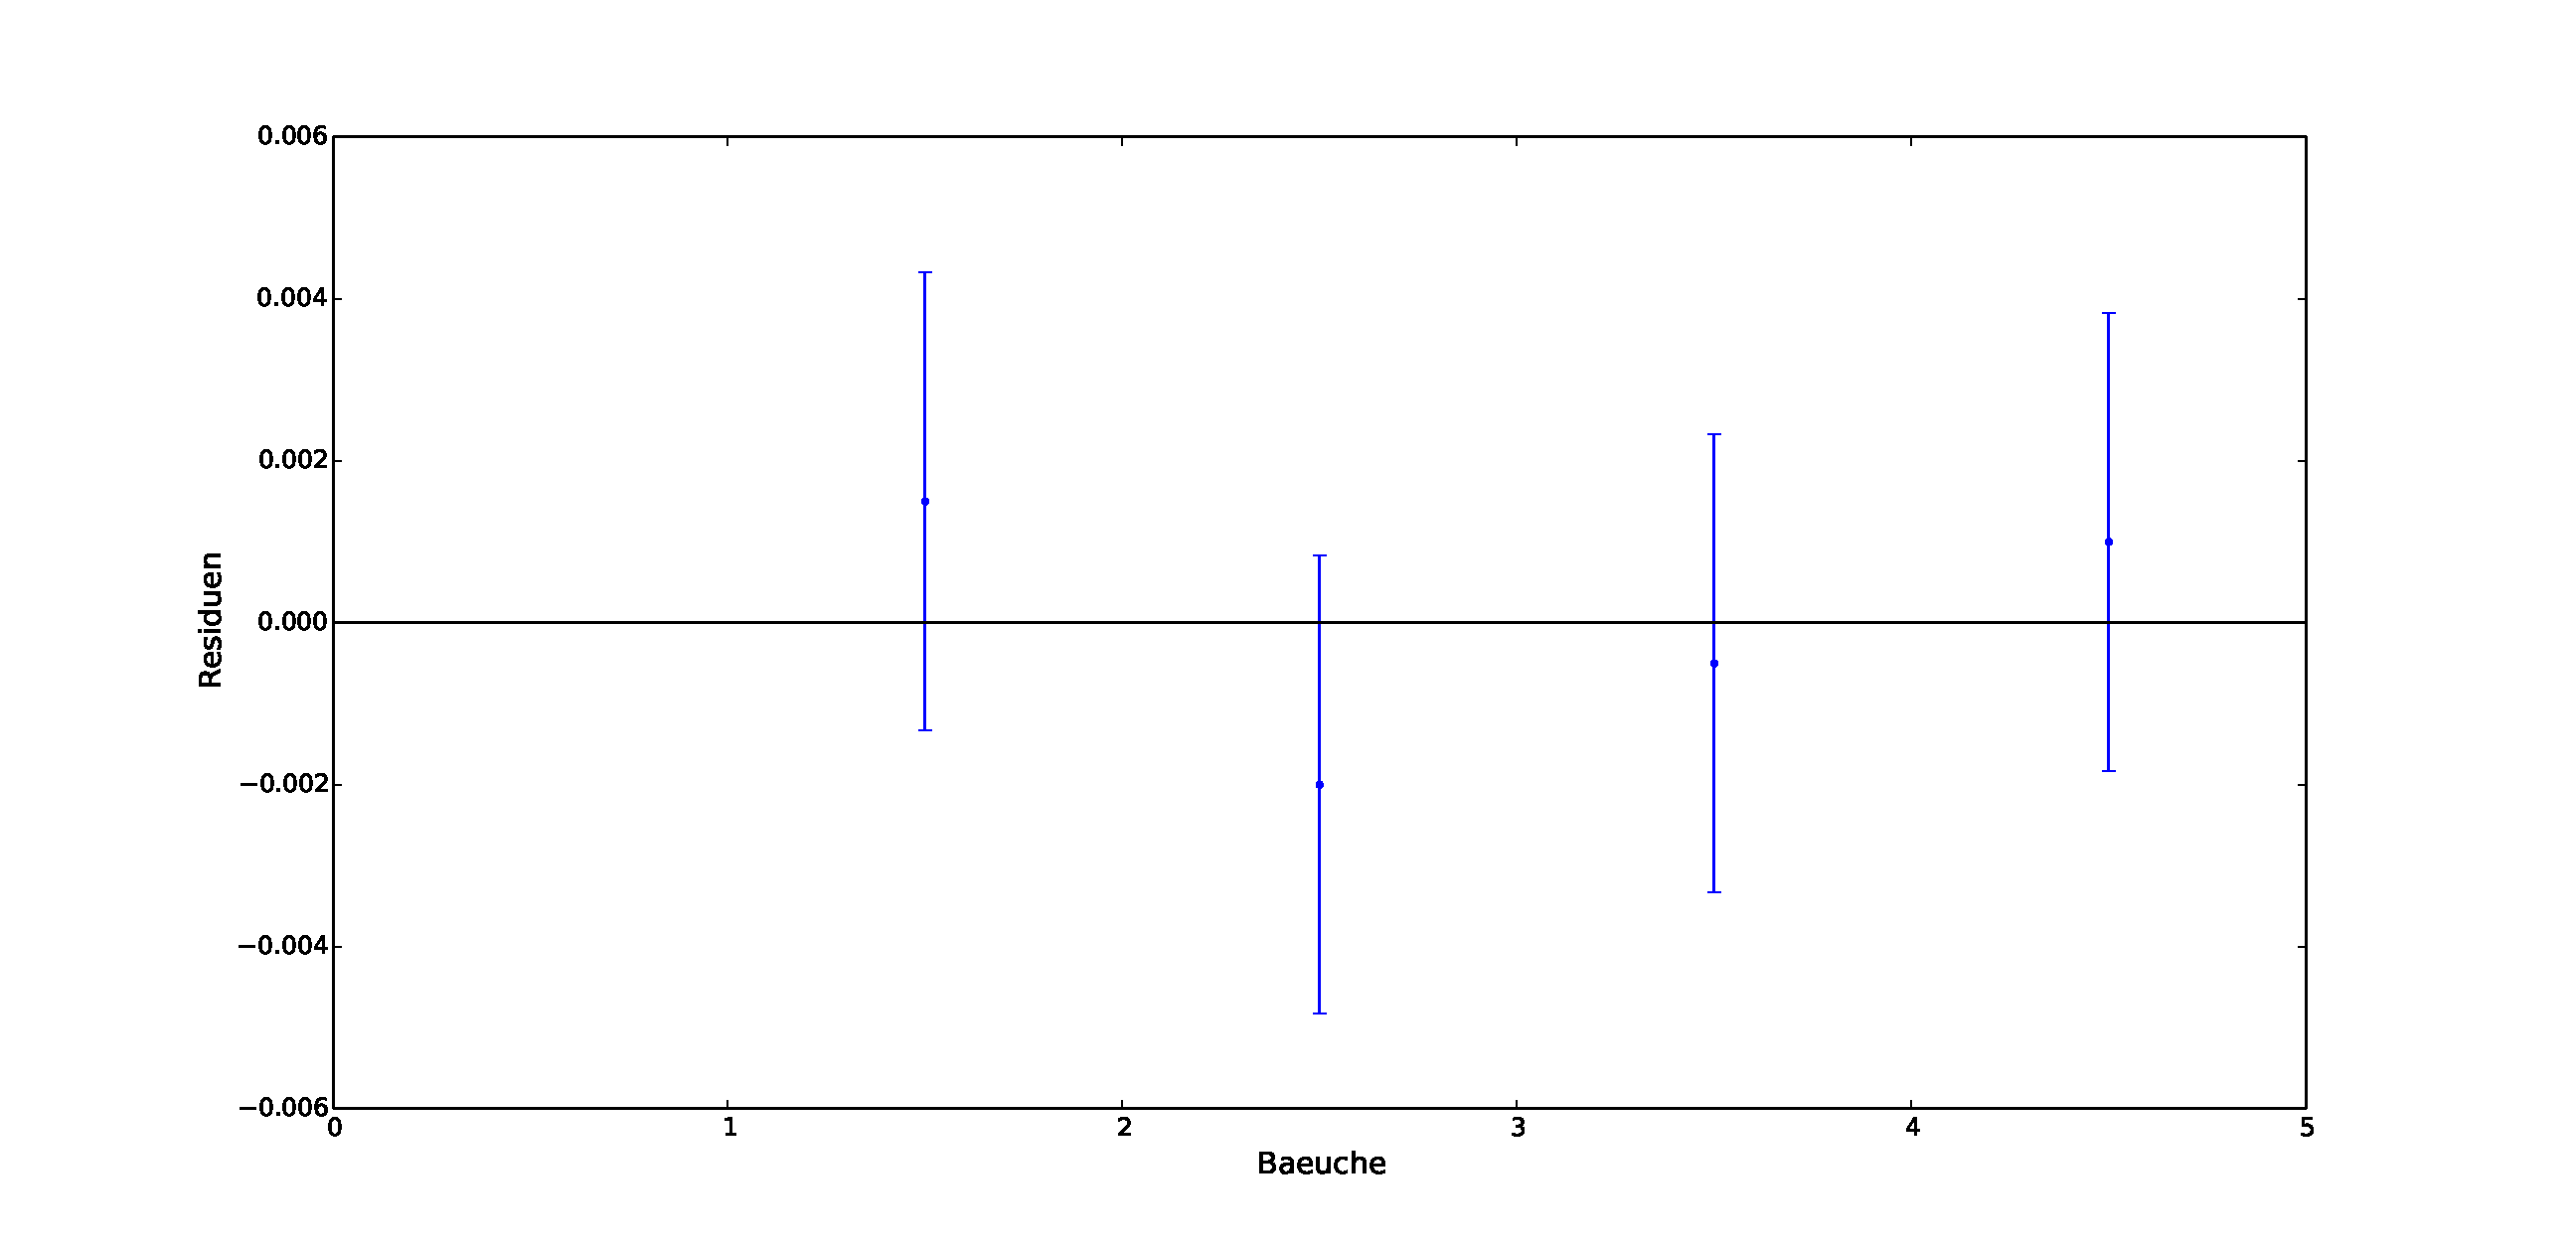
\includegraphics[scale=0.25]{Bilder/residuen_stehende_welle.eps}
\caption{Residuenplot (Daten - Fit) mit den jeweiligen Fehlern}
\end{figure}
\end{frame}

\begin{frame}{Fehlerrechnung und Ergebnis}
\begin{equation}
\sigma_{v} = \sqrt{f^2\cdot\sigma_{\lambda}^2 + \lambda^2\cdot\sigma_{f}^2}
\end{equation}
mit $\sigma_{\lambda} = 0.0025\,$m 
\begin{itemize}
\item $v = 352.8 \pm 4.5\,\frac{m}{s}$ 
\end{itemize}
\end{frame}

\section{Fazit}
\begin{frame}{Fazit}
\begin{itemize}
\item unser Wert: $v = 352.8 \pm 4.5\,\frac{m}{s}$ 
\item Literaturwert: $v = 344.98\,\frac{m}{s}$
\item Güte unserer Anpassung: $\frac{\chi^2}{f} = 0.47$
\end{itemize}
\end{frame}

\end{document}
